\chapter{Methodologies}
\label{cha:methodologies}


This chapter explains the methodologies used to address the research objectives
in this thesis. It describes the feature extraction and  engineering methods,
the use of explainable AI methods, model training and optimization approaches,
clustering and dimensionality reduction techniques and statistical hypothesis
testing methods.
%---------------------------------------------------------------------------

\section{Feature Engineering}
\label{sec:featureengineering}

Feature engineering is a critical step in the research process, as it involves
transforming raw data acquired using the data collection script into meaningful
representations that can be analyzed or used for predictive modeling. This
section describes the methodologies used to extract acoustic features from the
mp3 files and lyrical features from the lyrics. These features are designed to
capture key characteristics of the songs, enabling deeper insights into their
patterns and relationships.

\subsection{Acoustic Features}
\label{sec:acousticfeatures}

 These features provide a quantitative representation of the audio properties
 of each song and were extracted directly from the audio files in MP3 format.
 They describe various aspects of audio signal and provide insights into the
 rhythm, timbre, harmony and other acoustic properties. The extraction was done
 using \textit{Librosa}\cite{librosa} and was automated and parallelized to make it suitable
 for processing large amounts of data. 

\subsubsection*{MFCC - Mel Frequency Cepstral Coefficients}
MFCCs represent the short-term power spectrum of a song on a mel-scale and are
widely used for timbre analysis. These coefficients capture the tonal quality
of the audio and help differentiate between different instruments and vocal
characteristics.


\subsubsection*{Chroma}
Chroma vectors represent the intensity of each pitch class (e.g., C, C\#, D,
etc.) in the audio. These features provide a harmonic representation of the
song and are useful for analyzing chord progressions and harmonic structures.

\subsubsection*{Spectral Contrast}
Spectral contrast measures the difference in amplitude between peaks and
valleys in the spectrum. It provides insights into the harmonic and timbral
content of a song, particularly useful for distinguishing between smooth and
complex textures.

\subsubsection*{Other Features}
Two additional features were extracted:
\begin{itemize}
  \item \textbf{Tempo} - refers to the speed of the song, measured in
    \textit{Beats Per Minute(BPM)}
  \item \textbf{Zero Crossing Rate(ZCR)} - measures the rate at which the audio
    signal changes sign. It's commonly used as a measure of noisiness or
    percussive nature of signal
\end{itemize}

%---------------------------------------------------------------------------

\subsection{Lyrical Features}
\label{sec:lyricalfeatures}

Lyrical features  were extracted from the lyrics fetched during the data
collection process. They aim to provide a linguistic and semantic
representation of the track, capturing their complexity, sentiment and
stylistic  attributes. The cleaning and extraction  process utilized various
NLP libraries like \textit{NLTK}\cite{nltk}, \textit{spaCy}\cite{spacy} and
\textit{TextBlob}\cite{textblob}, alongside with custom ad-hoc algorithms.
Similarily to acoustic features the implementation allowed for simple and
intuitive usage under clear and comprehensible interface, with parallelization
of the computation process for increased performance. The features extracted
can be grouped as follows:

\subsubsection*{Basic Linguistic Metrics}
\begin{itemize}
  \item \textbf{Unique Word Count} - measures number of unique words in the
    lyrics, indicating diversity.
  \item \textbf{Type-Token Ratio} - a measure of lexical richness: ratio of
    unique words to total words.
  \item \textbf{Word Count} - total  number of words, baseline for text size
    and compexity.
  \item \textbf{Noun and Verb Ratios} - proportions of nous and vers relative
    to the total word count.
\end{itemize}


\subsubsection*{Sentiment and Emotional Tone}
\begin{itemize}
  \item \textbf{Sentiment Polarity} - a measure of overall sentiment(positive
    vs. negative) of the text.
  \item \textbf{Sentiment Subjectivity} - represents the degree of subjectivity
    in the lyrics, attempting to make a distinction between factual and
    opinionated content.
  \item \textbf{VADER Compound} - a sentiment score derived from the VADER
    tool.
  \item \textbf{Sentiment Variability} - standard deviation of sentiment on
    subsets of lyrics, a metric  aiming to capture fluctuations of sentiment
    throughout the song, highlighting emotional complexity.
\end{itemize}


\subsubsection*{Stylistic Features}
\begin{itemize}
  \item \textbf{Repetition Count} - the frequency of repeated words.
  \item \textbf{Rhyme Density} - a measure of how often rhymes occur in the
    text.
  \item \textbf{Linguistic Uniqueness} - ratio of rarely used words to all the
    words in the song.
\end{itemize}


\subsubsection*{Semantic and Complexity Features}
\begin{itemize}
  \item \textbf{Semantic Depth} - represents the richness and variety of
    meaning conveyed by the lyrics.
  \item \textbf{Syntactic Complexity} - captures the sophistication of
    sentence structures.
  \item \textbf{Lexical Richness} - quantifies the variety and richness of the
    vocabulary.
\end{itemize}



\subsubsection*{Readability and Accessibility}
\begin{itemize}
  \item \textbf{Flesch Reading Ease} - indicates how easy the lyrics are to
    read.
  \item \textbf{Gunning Fog} - a metric that estimates the  years of education
    required to understand the text.
  \item \textbf{Dale Chall} - a metric that accounts for familiar and
    unfamiliar words in the text.
\end{itemize}


\subsubsection*{Contextual Information}
  In process of feature extraction the \textbf{language} of lyrics was also
  identified using \textit{langdetect} library that uses a classification model
  to make predictions based on n-grams extracted from the text. The identified
  language was also used in the cleaning process, to remove songs  that
  weren't in English.

\subsubsection*{TF-IDF (Term Frequency - Inverse Document Frequency)}

TF-IDF\cite{tfidf} is a measure that can quantify the relevance of tokens in a
document amongst a collection of documents. In the context of this study, it
determines how important a word in a song's lyrics is  compared to all other
song's lyrics in the dataset. It's used to highlight words that are unique or
meaningful while giving less importance to very common words like 'the' or
'and'.

It can be broken down into two parts:


\begin{itemize}
  \item \textbf{TF - Term Frequency} - Measures the frequency of a term within
    a document:
  \[
  TF(w, d) = \frac{f_{w, d}}{N_d}
  \]
  where:
  \begin{itemize}
    \item \( f_{w, d} \): The number of times the word \( w \) appears in the
      document \( d \).
    \item \( N_d \): The total number of words in the document \( d \).
  \end{itemize}

  \item \textbf{IDF - Inverse Document Frequency} - Measures the rarity of a
    term across a collection of documents:
  \[
  IDF(w) = \log{\frac{N}{1 + n_w}}
  \]
  where:
  \begin{itemize}
    \item \( N \): The total number of documents in the corpus.
    \item \( n_w \): The number of documents containing the word \( w \).
  \end{itemize}
\end{itemize}

\subsubsection*{Word2Vec}

Word2Vec\cite{w2v} is a neural network-based technique for creating dense
vector representations of words, capturing their semantic relationships in a
high-dimensional space. Unlike traditional bag-of-words or TF-IDF methods,
Word2Vec generates embeddings that preserve the contextual meaning of words
based on their usage within the corpus.

Two primary approaches are used in Word2Vec: 
\begin{itemize} 
  \item \textbf{Continuous Bag of Words (CBOW)}: Predicts a target word based
    on its surrounding context words. 
  \item \textbf{Skip-Gram}: Predicts context words given a target word, better
    suited for capturing rare word relationships.
\end{itemize}

In this study, Word2Vec was used to create vector representations of song
lyrics. These embeddings enable the analysis of semantic relationships between
words, contributing to model performance in advanced tasks such as genre
classification, clustering, and thematic exploration.



\subsubsection*{Empath}
Empath\cite{empath} is a semantic analysis tool designed for extracting
semantic, thematic and emotional features from text by analyzing words based on
predefined categories. It classifies words into over 200 built-in categories,
such as \textit{sadness}, \textit{food} and \textit{music}. It  identifies
relationships between words and these categories, offering a higher-level
representation of text content beyond simple word frequency.

In this study, Empath was  used to analyze song lyrics, allowing for extraction
of thematic and  emotional content. These features were used to complement
other lyrical reprersentations, such as TF-IDF and Word2Vec. In contrary to
those methods however, empath provided a broader contextual understanding of
lyrics by summarizing them into measningful categories. This approach also
enhanced the interpretability of topics identified by LDA, as empath features
offered an additional layer of semantic insight, making it easier to
characterize and describe those topics.

Moreover, Empath allows for a more nuanced exploration of lyrical content
across different genres. By analyzing trends in emotional categories like
sadness or anger, and themes such as party or work, it helps to identify
meaningful variations between genres or time periods.

By combining Empath with traditional feature extraction methods, this study
benefits from a richer, more interpretable representation of lyrical content.


%---------------------------------------------------------------------------

\section{Explainable AI Methods}
\label{sec:explainableaimethods}


Explainable AI (XAI) techniques provide insights into the decision-making
processes of ML models, making it possible to understand the complex
relationships captured within the training data. By bridging the gap between
the pattern-recognition capabilities of these models and their practical
applications, XAI enables transparency and improves the interpretability of
results.

In this study this methodology was applied in various experiments to understand
how specific variables influence others, with aim of uncovering relationships
in the data and validating hypotheses. A deeper  understanding of factors
driving model predictions ensured that the results were both reliable and
meaningfully adressed the research objectives. The  techniques employed in this paper are: 

\subsubsection*{SHAP (SHapley Additive exPlanations)}
SHAP\cite{shap} values offer a detailed  breakdown of how individual features contribute
to  each prediction. It uses game theory principles to compute the importance
of each feature for a given output, providing both global insights on general
feature importance and  local explainations, showing how diffrenet features
contributed to specific predictions. In this study SHAP values were used in
order to explain the predictive process of trained Catboost models, allowing
for identification of key features for specific prediction task and
visualization of relationships.

\begin{center}
  \begin{figure}[H]
  \centering
  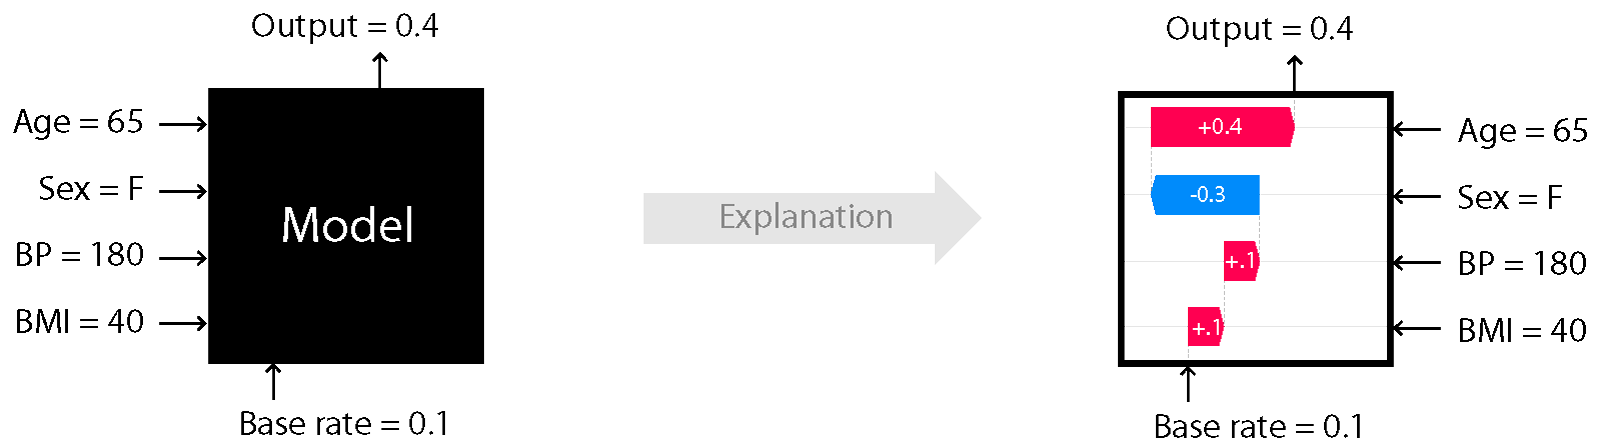
\includegraphics[width=4in]{img/shap_intro.png}
  \caption{SHAP\cite{shap}}
  \label{Figure:fig_beh}
\end{figure}
\end{center}

\begin{center}
  \begin{figure}[H]
  \centering
  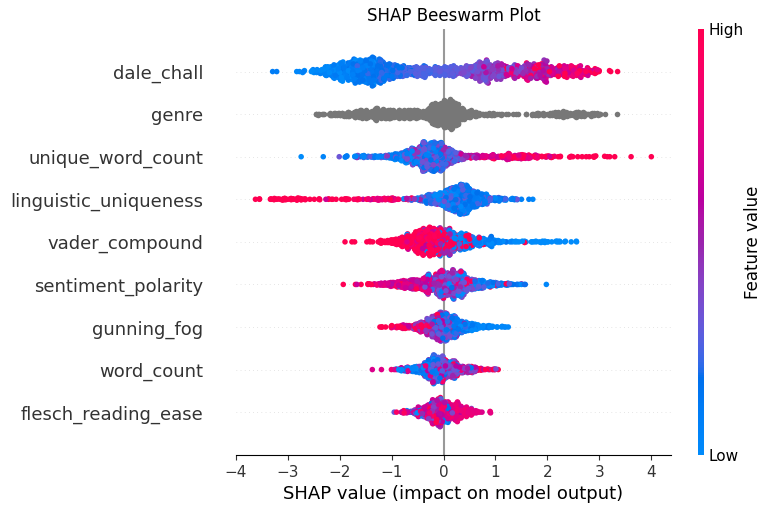
\includegraphics[width=4.5in]{img/shap_beeswarm.png}
  \caption{Example SHAP beeswarm plot showing impact of some lyrical features
  on the classifier of \textit{explicitness}.}
  \label{Figure:fig_beh}
\end{figure}
\end{center}

\begin{center}
\begin{figure}[H]
  \centering
  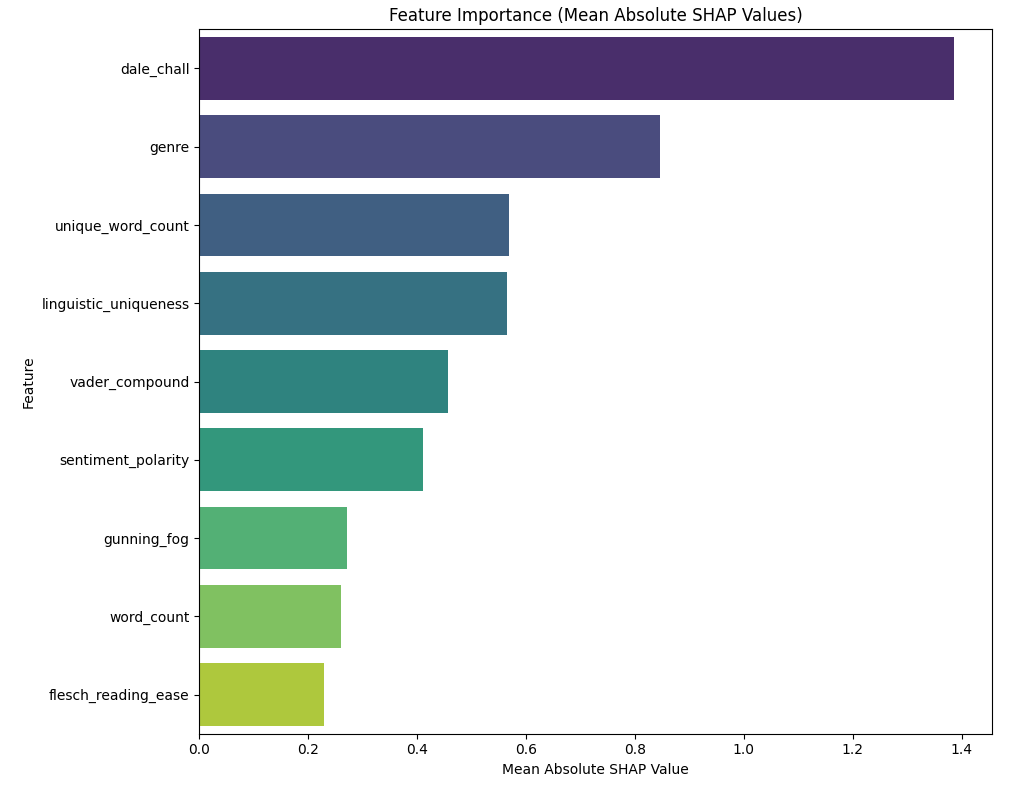
\includegraphics[width=3in]{img/shap_feature_importance.png}
  \caption{Example SHAP feature importance plot showing impact of some lyrical features
  on the classifier of \textit{explicitness}.}
  \label{Figure:fig_beh}
\end{figure}
\end{center}
%---------------------------------------------------------------------------

\subsubsection*{Machine Learning Models}
In this study, CatBoost\cite{catboost}, a widely recognized gradient boosting
algorithm known for its high predictive accuracy and efficiency, was employed
to build classification and regression models. These models utilized a
combination of acoustic, lyrical and metadata features in order to predict the
variable of interest, leveraging Catboost's strengths in handling diverse and
complex datasets. The result models were then subjected to SHAP analysis, in
order to understand their decision process and understand the interactions
between features and the target variable. Catboost was chosen for its
flexibility, ease of use, robust performance, compatibility with SHAP and
built-in support for categorical features,  which eliminated the need for
extensive preprocessing.

In order to further optimize the performance of these models, the
hyperparameter tuning library \textit{Optuna}\cite{optuna} was used. Its
efficient optimization framework allowed for systematic exploration of
different sets of hyperparameter configurations, ensuring the model achieved
optimal performance while avoiding overfitting. 

To address the challenges commonly encountered when training ML models on
complex datasets, following techniques were employed:
\begin{itemize}
  \item \textbf{Cross-validation} - cross-validation was used to reduce the
    risk of overfitting and provide reliable performance metrics. By dividing
    the data into multiple folds, the model was iteratively trained and
    validated on different subsets, therefore ensuring robust evaluation across
    the dataset and improved model's reliability, at the cost of increased
    computational time.
  \item \textbf{Class Weights} - to handle class imbalance in target variable
    labels, CatBoost offers a built-in capability to assign different penalties
    for misclassifications of specific classes. This adjustment improves
    model's ability to make accurate predictions across all classes, instead of
    favouring the majority class.
  \item \textbf{Out of sample evaluation} - model's performance was assessed on
    a separate test dataset that was excluded from the training. This step
    provided a reliable measure of model's ability to generalize on unseen data
    and ensured evaluation metrics  reflected its real predictive performance.
\end{itemize}

\section{Dimensionality Reduction - Principal Component Analysis (PCA)}
\label{sec:dimensionalityreduction}

Principal Component Analysis (PCA) reduces the number of features in large
datasets by transforming them into principal components that retain most of the
original information. It achieves this by converting potentially correlated
variables into a smaller set of less correlated variables, called principal
components, in a way that preserves as much of the original variance as
possible\cite{pca}. PCA is often employed to reduce dataset dimensionality and improve
generalization by reducing noise and redundancy in the data.

In this study, PCA was applied to the TF-IDF vectors derived from
song lyrics. TF-IDF vectors are typically high-dimensional, with thousands of
features representing individual terms across the corpus. Such high-dimensional
data can pose challenges, including increased computational complexity and a
higher risk of overfitting in machine learning models.

The use of PCA on these vectors reduced their dimensionality while preserving
as many significant patterns from the original vectors as possible. This
process improved computational efficiency and the interpretability of the data,
which is particularly important in the context of Explainable AI (XAI)
methodologies.

\begin{center}
\begin{figure}[H]
  \centering
  \includegraphics[width=4in]{img/pca.png}
  \caption{A scatterplot showing the relationship between PC1 and PC2 when PCA
  is applied to a dataset. PC1 and PC2 axis are perpendicular to each other.\cite{pca}}
  \label{Figure:fig_beh}
\end{figure}
\end{center}


\section{Topic Modelling - Latent Dirichlet Allocation (LDA)}
\label{sec:topicmodelling}

Latent Dirichlet Allocation (LDA)\cite{lda} is a generative probabilistic model
designed to uncover latent topics within a collection of discrete data, such as
text corpus.  It represents each document as a mixture of topics, where each
topic is characterized by a distribution over words. 

In this study, LDA was applied on the lyrics in order to identify commonly
ocurrirng topics in songs. Each song's lyrics were represented as a combination
of topics, and the most representative words for each topic were extracted.
This provided insights into the thematic content of lyrics, enabling further
exploration of relationships between lyrical topics and other features, like
popularity or acoustic properties.

By combining the topics derived with LDA with additional features, such as
acoustic parameters, the study aimed to analyze the interplay between a song's
musical and lyrical components.


\section{Statistical Methods}
\label{sec:statisticalmethods}

Statistical methods provided a foundation for analyzing complex relationships
between features and a framework for descriptive data analysis and hypothesis
testing.

\subsection{Pearson Correlation}

Pearson Correlation is a statistical measure used to quantify linear
relationship between two continuous variables. The resulting coefficient ranges
from -1 to 1 and is computed in the following way:

\[
r = \frac{\sum{(x_i - \bar{x})(y_i - \bar{y})}}{\sqrt{\sum{(x_i - \bar{x})^2} \sum{(y_i - \bar{y})^2}}}
\]

\noindent \noindent Where:
\begin{itemize}
    \item \( x_i \) and \( y_i \): The data points for the two variables.
    \item \( \bar{x} \) and \( \bar{y} \): The mean values of the variables.
\end{itemize}

\noindent \noindent Interpretation:
\begin{itemize}
  \item An \textit{r} value close to 1 indicates very strong positive linear
    relationship.
  \item An \textit{r} value close to -1 indicates very strong negative linear
    relationship.
  \item An \textit{r} value close to 0 indicates little to no relationship.
\end{itemize}



\subsection{Bootstrap Testing}

Bootstrap testing was used to verify hypotheses specified in the research
objectives. It's a resampling-based statistical technique that estimates the
variability of a statistic(e.g. mean or median)  by repeatedly sampling its
values from the dataset with replacement. It's highly versatile since it
doesn't rely on strong distributional assumptions.


\begin{center}
\begin{figure}[H]
  \centering
  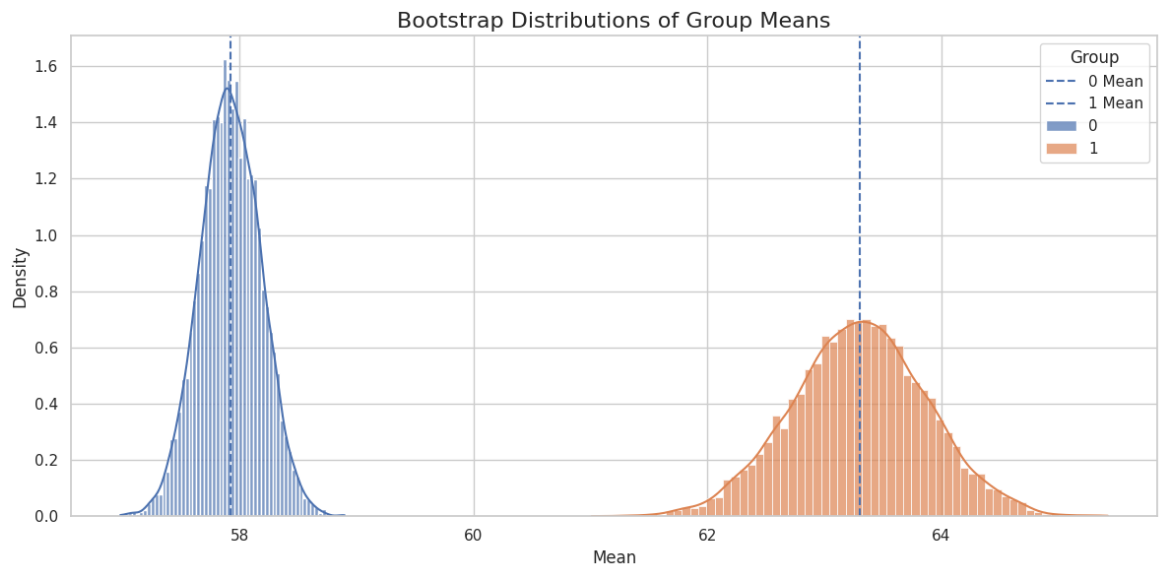
\includegraphics[width=5in]{img/bootstrap.jpg}
  \caption{Illustration of bootstrap resampling: The distribution of the
  statistic (e.g., mean) of the target variable for two different samples
(called groups). This demonstrates the variability of the statistic across
resampled datasets.}
  \label{Figure:fig_beh}
\end{figure}
\end{center}

\subsection{Analysis of Variance - ANOVA}
ANOVA is a statistical method used to compare the means of three or more groups
to determine if there is a statistically significant difference among them. It
tests the hypothesis that the means of all groups are equal against the
alternative hypothesis that at least one group mean is different.

\subsubsection*{Hypotheses}
\begin{itemize}
  \item \textbf{Null Hypothesis($H_0$)}: All group means are equal.
  \item \textbf{Alternative Hypothesis($H_a$)}: At least one group mean is
    different.
\end{itemize}

\noindent \noindent In order to verify the hypotheses, two types of variation are calculated:

\subsubsection*{Between-Group Variation}

This type of variation measures the differences between the means of groups. It
captures how much the group means differ from the overall mean.
\[
\text{Between-group \  variation} = \sum_{i=1}^{k} n_i (\bar{x}_i - \bar{x})^2
\]

\noindent \noindent Where:
\begin{itemize}
    \item \(n_i\): Number of samples in group \(i\).
    \item \(\bar{x}_i\): Mean of group \(i\).
    \item \(\bar{x}\): Overall mean.
\end{itemize}


\subsubsection*{Within-Group Variation}
It measures the variability of data points within each group.

\[
\text{Within-group  \ variation} = \sum_{i=1}^{k} \sum_{j=1}^{n_i} (x_{ij} - \bar{x}_i)^2
\]

\noindent \noindent Where:
\begin{itemize}
    \item \(x_{ij}\): Individual data point in group \(i\).
    \item \(\bar{x}_i\): Mean of group \(i\).
\end{itemize}



\subsubsection*{F-Statistic Calculation}
In order to calculate the \textbf{F-statistic} and verify the hypotheses
the MSB and MSW have to be calculated:

\begin{itemize}
    \item \textbf{Mean Square Between (MSB)}:
    
    Formula:
    \[
    \text{MSB} = \frac{\text{Between-group variation}}{\text{df}_{\text{between}}}
    \]
    \noindent \noindent Where:
    \begin{itemize}
        \item \( \text{df}_{\text{between}} = k - 1 \): Number of groups minus one.
    \end{itemize}
\end{itemize}

\begin{itemize}
    \item \textbf{Mean Square Within (MSW)}:
    
    Formula:
    \[
    \text{MSW} = \frac{\text{Within-group \ variation}}{\text{df}_{\text{within}}}
    \]
    \noindent \noindent Where:
    \begin{itemize}
        \item \( \text{df}_{\text{within}} = N - k \): Total number of observations minus the number of groups.
    \end{itemize}
\end{itemize}


The \textbf{F-statistic} is calculated as the ratio of between-group variance
to within-group variance:
\[
F = \frac{\text{MSB}}{\text{MSW}}
\]


Based on the calculated F-statistic, p-value can be calculated and depending on
the value and the chosen significance level the null hypothesis $H_0$ will be
rejected or not.
